% Provenance (never printed): see sources/outline_sources.md (Year 3: gravity, magnetic,
% seismic, resistivity and ground-penetrating-radar surveys; data processing and
% uncertainty; a mapping project).
% Brief: sources/book5/BRIEFS.md, ch. 31. Curves from figdata/bachelor-3/gravity_granite.py
% (prism model of the Varden granite of figdata/shared/region.py), magnetic_dyke.py (2-D
% dyke; the Varden dolerite dyke of the Sync 3 ruling, buried below the unconformity),
% resistivity_sounding.py (Pekeris transform and image series) and gpr_radargram.py.
% Physical-property ranges and survey practice from the GPG open textbook (CC BY 4.0) and
% Keys (1990). Exercise and problem values in the Book 5 scratch calculator calc/ch31.py.
\chapter{Métodos de campo e de laboratório III}\label{ch:b3:field-lab-methods-3}

Uma equipe de geofísica passa uma semana no vale de Varden Hills, a
região fictícia cujo mapa geológico o volume do primeiro ano desenhou em
seu capítulo sobre mapas geológicos. O mapa mostra um granito aflorando nas
encostas do vale, entre os xistos, sob o arenito que
repousa sobre ambos. Onde o granito segue sob a cobertura, até onde
se estende e até que profundidade alcança, ninguém viu. A equipe leva um
gravímetro, dois magnetômetros, um cabo de eletrodos e um radar sobre um
carrinho pequeno. Nenhum desses instrumentos enxerga uma rocha: cada um mede um
campo na superfície---gravidade, o campo magnético, um
potencial elétrico, o eco de um pulso de rádio---que as rochas abaixo perturbam.
Ao fim da semana, a equipe consegue desenhar o granito que nunca viu, dizer
quão profundo é o aluvião do fundo do vale e relatar um corpo magnético
que nenhum mapa mostrava.

Este capítulo acompanha essa semana. Ele trata cada método em sequência, como
uma medida com suas correções e como um \omterm{def:b3:seismology-imaging:inverse}{problema direto} com alguns corpos cujos
campos podem ser calculados exatamente; depois, expõe-se como os erros de um
levantamento se somam e por que um único tipo de dado raramente determina um
modelo; e termina com o levantamento de Varden, em que os métodos são
reunidos.

\begin{recall}
A anomalia da gravidade, as correções de ar livre e de Bouguer e suas anomalias
e a gravidade normal estão no volume do primeiro ano, em seu capítulo sobre
isostasia e gravidade; o ciclo de levantamento de um \omterm{def:b3:field-lab-methods-3:gravimeter}{gravímetro relativo} é
descrito no \cref{ch:b3:gravity-geodesy}. O campo principal, sua inclinação, a
\omterm{thm:b3:palaeomagnetism:dipole}{fórmula do dipolo} e o \omterm{def:b3:palaeomagnetism:igrf}{Campo Geomagnético Internacional de Referência} estão
no \cref{ch:b3:palaeomagnetism}. Resistividade, lei de Ohm, a permissividade
relativa, as ondas eletromagnéticas, a magnetização e a
suscetibilidade magnética estão nos livros de física, e o teorema de Gauss para
a gravidade, junto com eles. Os \omterm{def:b3:exploration-seismology:surveys}{levantamentos de refração sísmica} estão no
\cref{ch:b3:exploration-seismology}; \omterm{def:b3:seismology-imaging:inverse}{problemas diretos} e inversos e mínimos
quadrados ponderados estão no \cref{ch:b3:seismology-imaging}; a porosidade, nos
volumes escolares, e os perfis a cabo, no \cref{ch:b3:facies-models}. A
propagação de incertezas está nos livros de química e de matemática.
\end{recall}

\section{Levantamentos gravimétricos}\label{sec:b3:field-lab-methods-3:gravity}

As anomalias que um levantamento gravimétrico procura são pequenas. A gravidade no
equador é de cerca de \qty{978000}{\milli\gal}; grandes estruturas a alteram
em centenas de miligals, um domo de sal em cerca de dez, um corpo de minério em
cerca de um, e os alvos de um levantamento geotécnico em alguns
centésimos. Geofísicos medem em
miligals, ou em unidades de gravidade de \qty{0.1}{\milli\gal}; um levantamento
útil precisa resolver diferenças de uma parte em cem milhões de~$g$.
% ledger: gpg:grav-units, gpg:grav-sizes

\begin{definition}[Gravímetro relativo; deriva instrumental]\label{def:b3:field-lab-methods-3:gravimeter}
Um \emph{gravímetro relativo}\index{gravímetro relativo} é um
instrumento que mede diferenças de gravidade entre estações: uma massa presa a
uma mola, mantida em posição nula por uma segunda força ajustável, cuja
leitura no mostrador, multiplicada por uma constante de calibração, fornece a gravidade
em miligals, a menos de uma constante desconhecida. Sua \emph{deriva
instrumental}\index{deriva instrumental} é a lenta variação de sua leitura em uma
estação fixa, causada pela fluência da mola, pela temperatura e por choques;
mede-se relendo, após algumas horas, uma
estação já lida, a \emph{estação-base}.
\end{definition}
% ledger: gpg:gravimeter, gpg:grav-survey

Um gravímetro de campo cobre uma faixa de várias dezenas de milhares de
miligals e lê, em seu melhor, cerca de \qty{0.01}{\milli\gal}; a faixa deve ser
reiniciada após o transporte. Nessa precisão, a altura de cada estação importa
tanto quanto sua leitura: \qty{3.3}{cm} de erro de altura compromete
\qty{0.01}{\milli\gal}, por isso as posições são levantadas com receptores de
satélite ou com um nível, com precisão de centímetro. A estação-base é
reocupada a cada duas horas. A maré terrestre sólida, que pode chegar a
\qty{0.3}{\milli\gal}, muda lentamente o bastante nessas horas para ser
removida junto com a deriva.
% ledger: gpg:gravimeter, gpg:grav-survey, gpg:grav-sizes

\begin{method}[Redução de um ciclo gravimétrico]\label{met:b3:field-lab-methods-3:loop}
Um ciclo começa e termina em uma estação-base, lida nos instantes $t_0$ e $t_1$.
\begin{enumerate}
  \item Calcula-se a taxa de deriva $(r_1 - r_0)/(t_1 - t_0)$ a partir das duas
        leituras da base; ela inclui a maré.
  \item Subtrai-se de cada leitura a deriva acumulada desde $t_0$,
        $r - (t - t_0)(r_1 - r_0)/(t_1 - t_0)$, e subtrai-se a leitura da base:
        isso é a gravidade relativa à base.
  \item Corrige-se pela altura $\Delta h$ da estação acima da base:
        soma-se a correção de ar livre $\qty{0.3086}{\milli\gal.m^{-1}}
        \times\Delta h$ e subtrai-se a correção de Bouguer
        $\qty{0.1119}{\milli\gal.m^{-1}}\times\Delta h$ (densidade
        \qty{2670}{kg.m^{-3}}), isto é, soma-se $0.1967\,\Delta h$.
  \item Para uma estação a uma distância $\Delta y$ ao norte da base, subtrai-se
        a variação da gravidade normal, $\qty{0.811}{\milli\gal.km^{-1}}
        \times\sin 2\varphi\times\Delta y$.
  \item Soma-se a \omterm{def:b3:field-lab-methods-3:terrain}{correção de terreno} de cada estação.
\end{enumerate}
O resultado é a anomalia de Bouguer relativa à base. Amarrar a base a uma
estação de gravidade absoluta conhecida fornece a própria anomalia.
\end{method}
% ledger: gpg:grav-survey, gpg:terrain

A correção de Bouguer trata o terreno entre a estação e o nível de referência
como uma laje plana. Em um relevo real, isso está errado de duas maneiras:
um morro que se eleva acima da estação puxa para cima e reduz a leitura, e
um vale que cai abaixo dela é contado na laje como uma rocha que
não está lá.

\begin{definition}[Correção de terreno]\label{def:b3:field-lab-methods-3:terrain}
A \emph{correção de terreno}\index{correção de terreno} de uma estação
de gravidade é a atração que os desvios do relevo em relação à
laje de Bouguer exercem sobre ela: os morros acima do nível da estação, e
os vales abaixo dele, contados com a densidade da laje. Ambos reduzem
a gravidade medida em comparação com a laje, por isso a correção é
sempre somada.
\end{definition}

Ela era calculada à mão, com um ábaco de Hammer e tabelas, zona por zona
afastando-se da estação; hoje ela é calculada a partir de um modelo digital
de elevação. Longe de relevos íngremes, ela raramente excede \qty{1}{\milli\gal},
mas as zonas próximas à estação são difíceis de acertar, e a
correção raramente é conhecida com precisão melhor que \qty{0.2}{\milli\gal}.
% ledger: gpg:terrain, gpg:grav-sizes

\subsection{Anomalias de corpos simples}

O \omterm{def:b3:seismology-imaging:inverse}{problema direto} da gravidade é uma soma: cada elemento de um corpo de
contraste de densidade $\Delta\rho$ atrai a estação pela lei de Newton, e
um levantamento mede a componente vertical da soma. Alguns corpos admitem
solução em forma fechada.

\begin{theorem}[Esfera e cilindro horizontal]\label{thm:b3:field-lab-methods-3:sphere}
A uma distância horizontal $x$ do ponto acima de seu centro, uma esfera
enterrada de excesso de massa $\Delta m$, cujo centro está à profundidade $z$, fornece a
anomalia
\[
\Delta g(x) = \frac{G\,\Delta m\,z}{(x^2 + z^2)^{3/2}} ,
\]
e a anomalia cai à metade de seu pico em $x_{1/2} = z\sqrt{2^{2/3} - 1}$,
de modo que $z = 1.305\,x_{1/2}$. Um cilindro horizontal longo de excesso de massa
$\lambda$ por unidade de comprimento, com eixo à profundidade $z$, fornece, transversalmente à sua
direção
\[
\Delta g(x) = \frac{2G\lambda z}{x^2 + z^2} ,
\]
e $z = x_{1/2}$.
\end{theorem}

\begin{proof}
Fora de uma esfera cuja densidade depende apenas da distância ao seu
centro, a atração é a de sua massa concentrada no centro (o
teorema das cascas, consequência do teorema de Gauss). Sua intensidade na
estação é $G\Delta m/(x^2 + z^2)$, e a componente vertical carrega o
fator $z/\sqrt{x^2 + z^2}$. Escrevendo $\Delta g(x_{1/2}) =
\Delta g(0)/2$ obtém-se $(1 + x_{1/2}^2/z^2)^{3/2} = 2$, daí a regra. Para
o cilindro, o teorema de Gauss aplicado a um cilindro coaxial de raio $r$ fornece
um campo $2G\lambda/r$, e a componente vertical $2G\lambda z/r^2$;
metade do pico é atingida quando $x^2 + z^2 = 2z^2$.
\end{proof}
% ledger: gpg:half-width

Um corpo que não é uma esfera ainda tem uma meia-largura, e a regra então
fornece a profundidade de uma esfera equivalente, e não a do corpo. A regra é
uma primeira estimativa, feita antes de qualquer modelo ser ajustado.

\begin{proposition}[Cilindro vertical sobre seu eixo]\label{prop:b3:field-lab-methods-3:vcyl}
Um cilindro vertical de raio $a$ e contraste de densidade $\Delta\rho$,
cujos topo e base estão às profundidades $z_1 < z_2$ abaixo da estação,
fornece sobre seu eixo
\[
\Delta g = 2\pi G\Delta\rho\left[(z_2 - z_1) + \sqrt{z_1^2 + a^2}
           - \sqrt{z_2^2 + a^2}\right] .
\]
Para $a \to \infty$ trata-se da laje de Bouguer $2\pi G\Delta\rho(z_2 - z_1)$;
para um cilindro da superfície a grande profundidade, ela tende a
$2\pi G\Delta\rho\,a$.
\end{proposition}

\begin{proof}
Um disco de raio $a$ e espessura $\mathrm{d}z$ à profundidade $z$ atrai
um ponto sobre seu eixo com $2\pi G\Delta\rho\,\mathrm{d}z\,(1 -
z/\sqrt{z^2 + a^2})$, a atração de um anel integrada sobre o
raio. Integrando de $z_1$ a $z_2$ obtém-se o colchete. Quando $a \to
\infty$ com profundidades fixas, $\sqrt{z_1^2 + a^2} - \sqrt{z_2^2 + a^2} =
(z_1^2 - z_2^2)/(\sqrt{z_1^2 + a^2} + \sqrt{z_2^2 + a^2}) \to 0$; quando
$z_1 = 0$ e $z_2 \to \infty$, $z_2 - \sqrt{z_2^2 + a^2} \to 0$ e
o colchete tende a $a$.
\end{proof}

\begin{proposition}[Excesso de massa a partir de um mapa gravimétrico]\label{prop:b3:field-lab-methods-3:gauss}
Qualquer que seja a forma de um corpo que se situa inteiramente abaixo de um
plano horizontal, seu excesso de massa é
\[
\Delta m = \frac{1}{2\pi G}\iint \Delta g\,\mathrm{d}A ,
\]
a integral estendendo-se a todo o plano.
\end{proposition}

\begin{proof}
Para uma massa pontual $m$ à profundidade $z$, sendo $r$ a distância horizontal,
$\iint \Delta g\,\mathrm{d}A = \int_0^\infty
Gmz\,(r^2 + z^2)^{-3/2}\,2\pi r\,\mathrm{d}r = 2\pi Gm$: metade do fluxo
$4\pi Gm$ do teorema de Gauss atravessa o plano. Um corpo é uma soma de
massas pontuais, e a integral é linear.
\end{proof}

O teorema fornece a massa, nunca a forma; e um mapa cobre apenas parte
do plano, enquanto a anomalia de um corpo profundo decai lentamente, de modo que a
massa obtida de um mapa é pequena demais, a menos que suas bordas sejam estendidas por
um modelo.

\begin{omfigure}
\begin{tikzpicture}
\begin{axis}[axis equal image, xmin=1.5, xmax=5.5, ymin=2.6, ymax=5.7, width=0.86\linewidth,
  tick label style={font=\scriptsize}, xlabel={leste (km)}, ylabel={norte (km)},
  label style={font=\small}, unbounded coords=jump]
% geology of the region (figdata/shared/region.py), faded
\addplot[lith schist, draw=black!50, line width=0.2pt, even odd rule, opacity=0.45] table {figdata/out/shared-region-unit-schist.dat};
\addplot[lith granite, draw=black!50, line width=0.2pt, even odd rule, opacity=0.45] table {figdata/out/shared-region-unit-granite.dat};
\addplot[om lith={icsTriassic!35}{om sand}, draw=black!50, line width=0.2pt, even odd rule, opacity=0.45] table {figdata/out/shared-region-unit-sandstone.dat};
\addplot[om lith={icsJurassic!40}{om limestone}, draw=black!50, line width=0.2pt, even odd rule, opacity=0.45] table {figdata/out/shared-region-unit-limestone.dat};
\addplot[om lith={icsJurassic!15}{om shale}, draw=black!50, line width=0.2pt, even odd rule, opacity=0.45] table {figdata/out/shared-region-unit-shale.dat};
\addplot[lith alluvium, draw=black!50, line width=0.2pt, even odd rule, opacity=0.45] table {figdata/out/shared-region-unit-alluvium.dat};
\addplot[river] table {figdata/out/shared-region-river.dat};
% the survey (figdata/bachelor-3/gravity_granite.py, magnetic_dyke.py)
\addplot[only marks, mark=*, mark size=0.7pt, black!70] table[x=x_km, y=y_km] {figdata/out/bachelor-3-gravity_granite-stations.dat};
\addplot[omDef, very thick] table[x=x_km, y=y_km] {figdata/out/bachelor-3-gravity_granite-contours.dat};
\addplot[omThm, thick] coordinates {(1.5,4.15) (5.5,4.15)};
\addplot[omMeth, line width=2.2pt, opacity=0.8] coordinates {(1.7,4.15) (2.7,4.15)};
\addplot[omProp, dashed, thick] coordinates {(2.2,2.6) (2.2,5.7)};
\addplot[only marks, mark=star, mark size=3.5pt, omMeth!70!black, thick] coordinates {(3.5,4.0)};
\node[font=\scriptsize, fill=white, fill opacity=0.85, text opacity=1, inner sep=1pt] at (axis cs:3.5,5.12) {$-0.5$};
\node[font=\scriptsize, fill=white, fill opacity=0.85, text opacity=1, inner sep=1pt] at (axis cs:3.5,4.84) {$-1$};
\node[font=\scriptsize, fill=white, fill opacity=0.85, text opacity=1, inner sep=1pt] at (axis cs:3.5,4.58) {$-2$};
\node[font=\scriptsize, anchor=south west, fill=white, fill opacity=0.85, text opacity=1, inner sep=1pt] at (axis cs:1.55,4.17) {perfil gravimétrico};
\node[font=\scriptsize, anchor=north, fill=white, fill opacity=0.85, text opacity=1, inner sep=1pt] at (axis cs:2.2,4.08) {linha magnética};
\node[font=\scriptsize, anchor=north west, text=omProp!80!black, fill=white, fill opacity=0.85, text opacity=1, inner sep=1pt] at (axis cs:2.24,5.6) {dique enterrado};
\node[font=\scriptsize, anchor=north, fill=white, fill opacity=0.85, text opacity=1, inner sep=1pt] at (axis cs:3.5,3.92) {sondagem};
\pic at (axis cs:5.15,5.3) {northarrow};
\end{axis}
\end{tikzpicture}

\par\smallskip{\small O levantamento de Varden sobre o mapa geológico da região
(desbotado: xisto cinza, granito rosa, arenito, calcário e folhelho da cobertura,
aluvião ao longo do rio). Pontos pretos: as estações gravimétricas,
\qty{200}{m} de distância; azul: a anomalia de Bouguer do modelo do granito,
com isolinhas a cada \qty{0.5}{\milli\gal}; vermelho: o perfil gravimétrico; verde:
a linha magnética e a sondagem elétrica (estrela) no fundo do vale;
laranja tracejado: o dique de diabásio que o levantamento magnético encontra,
enterrado sob a cobertura.}\label{fig:b3:field-lab-methods-3:survey}
\end{omfigure}
% ledger: gpg:densities

\subsection{O granito de Varden}

O modelo do granito adotado pelos geólogos é um corpo elíptico abaixo da
discordância, com \qty{760}{m} de extensão leste--oeste e \qty{1120}{m}
norte--sul onde encontra a cobertura, alargando-se para baixo; nos
flancos do vale ele chega à superfície. O granito é mais leve que o xisto:
as faixas de densidade publicadas são \numrange{2.50}{2.81} e
\qtyrange{2.39}{2.80}{g.cm^{-3}}. O modelo do levantamento adota
\qty{2620}{kg.m^{-3}} para o granito e \qty{2750}{kg.m^{-3}} para o
xisto, um contraste de \qty{-130}{kg.m^{-3}}, e limita o granito a
\qty{1500}{m} abaixo do nível do mar, uma suposição, já que nada mostra sua
base. Dividido em \num{5533} prismas retos cujas atrações têm forma fechada,
o modelo fornece a anomalia do mapa acima: um mínimo fechado de
\qty{-2.29}{\milli\gal} sobre o centro do granito, com isolinhas
alongadas norte--sul, como o corpo.
% ledger: gpg:densities

\begin{omfigure}
\begin{tikzpicture}
\begin{axis}[width=0.8\linewidth, height=0.42\linewidth, xmin=1.5, xmax=5.5, ymin=-2.6, ymax=0.2,
  xlabel={leste (km)}, ylabel={$\Delta g$ (\unit{\milli\gal})},
  tick label style={font=\scriptsize}, label style={font=\small},
  legend style={font=\scriptsize, at={(0.02,0.04)}, anchor=south west}]
% computed in figdata/bachelor-3/gravity_granite.py
\addplot[omDef, very thick] table[x=x_km, y=dg_mGal] {figdata/out/bachelor-3-gravity_granite-profile.dat};
\addlegendentry{modelo do granito}
\addplot[omThm, densely dashed, thick] table[x=x_km, y=sphere] {figdata/out/bachelor-3-gravity_granite-profile.dat};
\addlegendentry{esfera da regra da meia-largura}
\addplot[omMeth, densely dotted, thick] table[x=x_km, y=cyl] {figdata/out/bachelor-3-gravity_granite-profile.dat};
\addlegendentry{cilindro vertical}
\addplot[black!40, forget plot] coordinates {(1.5,0) (5.5,0)};
\addplot[black!50, densely dotted, forget plot] coordinates {(1.5,-1.1464) (5.5,-1.1464)};
\node[font=\scriptsize, black!60, anchor=south east] at (axis cs:5.45,-1.14) {metade do pico};
\end{axis}
\end{tikzpicture}

\par\smallskip{\small A anomalia ao longo do perfil gravimétrico (azul), a
esfera cuja profundidade e massa a regra da meia-largura fornece (vermelho tracejado), e
um cilindro vertical da mesma área do granito na discordância,
desde o solo até a base do modelo (verde pontilhado). A esfera coincide
com o pico e a meia-largura por construção, mas não com os flancos; o
cilindro, que ignora o alargamento do corpo, fica aquém no
centro.}\label{fig:b3:field-lab-methods-3:profile}
\end{omfigure}
% ledger: gpg:half-width

\section{Levantamentos magnéticos}\label{sec:b3:field-lab-methods-3:magnetics}

O campo principal da Terra é de cerca de \qty{25000}{nT} no equador magnético
e de cerca de \qty{70000}{nT} próximo aos polos magnéticos. Rochas que contêm
magnetita somam ao campo seu próprio campo, induzido pelo campo principal em
proporção à sua suscetibilidade, ou remanente, adquirida no momento em que se formaram.
Uma rocha ígnea félsica tem suscetibilidade abaixo de cerca de
\num{2e-3}, e uma máfica, de cerca de \num{2e-3} a \num{0.4}; na mesma
escala, um por cento de magnetita em volume dá cerca de \num{0.03}.
% ledger: gpg:mag-field, gpg:susceptibility

\begin{definition}[Anomalia de campo total; correção diurna; redução ao polo]\label{def:b3:field-lab-methods-3:magnetic}
Seja $\mathbf{F}$ o campo principal no levantamento e $\Delta\mathbf{B}$
o campo das rochas magnetizadas.
\begin{itemize}
  \item A \emph{anomalia de campo total}\index{anomalia de campo total} é
        a intensidade medida menos a do campo principal, $\Delta T =
        |\mathbf{F} + \Delta\mathbf{B}| - |\mathbf{F}|$; quando
        $|\Delta\mathbf{B}| \ll |\mathbf{F}|$ ela é a projeção
        $\Delta\mathbf{B}\cdot\mathbf{F}/|\mathbf{F}|$.
  \item A \emph{correção diurna}\index{correção diurna} remove
        as variações do campo com o tempo: um magnetômetro em uma
        estação-base fixa registra o campo durante todo o levantamento, e cada
        leitura $T(t)$ do instrumento em movimento é substituída por $T(t) -
        T_\mathrm{base}(t)$.
  \item A \emph{redução ao polo}\index{redução ao polo}
        calcula, a partir da anomalia medida, a anomalia que as mesmas rochas
        produziriam se o campo principal fosse vertical, como em um
        polo magnético; a anomalia fica então posicionada acima de sua fonte.
\end{itemize}
\end{definition}
% ledger: gpg:mag-survey, gpg:mag-processing

As variações com o tempo vêm de correntes na ionosfera, a cerca de
\qty{110}{km} de altitude. Em um dia, elas somam tipicamente algo entre
\qtyrange{20}{50}{nT}, tanto quanto a anomalia de um alvo pequeno; uma
tempestade magnética pode alterar o campo em milhares de nanoteslas. A
estação-base mede a variação, na suposição de que ela seja a
mesma em todo o levantamento. O próprio campo principal, ou o campo de
estruturas maiores que o levantamento, é removido com o IGRF, uma constante
ou uma tendência ajustada.
% ledger: gpg:mag-field, gpg:mag-processing

Um magnetômetro de precessão de prótons mede a frequência com que os spins de prótons
precessam no campo, frequência essa proporcional ao campo; ele
lê até \qty{1}{nT} e precisa de mais de um segundo por leitura. Um
magnetômetro de césio bombeado opticamente é de dez a cem vezes mais
sensível, lendo até \qty{0.01}{nT}. As estações devem estar próximas o bastante
para colocar pelo menos cerca de três leituras ao longo da meia-largura da
anomalia mais estreita que se procura, e quanto mais rasa a fonte, mais próximas
devem estar.
% ledger: gpg:mag-survey

\begin{proposition}[Anomalia de um dique delgado]\label{prop:b3:field-lab-methods-3:dyke}
Um dique vertical de espessura $t$ e suscetibilidade $\kappa$, de direção
ao longo do meridiano magnético, com o topo à profundidade $z$ e estendendo-se
em profundidade, magnetizado por indução em um campo principal $F$ de inclinação $I$,
produz, transversalmente à direção, se $t \ll z$,
\[
\Delta T(x) = \frac{\kappa F t\sin^2 I}{2\pi}\,\frac{z}{x^2 + z^2} ,
\]
uma anomalia simétrica que cai à metade de seu pico em $x = \pm z$: a
profundidade do topo do dique é a metade da largura total da anomalia
medida à metade do pico.
\end{proposition}

\begin{proof}
O dique é bidimensional e o campo principal está no plano vertical
que contém a direção. A magnetização $\mathbf{M} = \kappa\mathbf{F}/\mu_0$
tem uma componente ao longo da direção, cujos polos ficam nas extremidades do
dique, distantes, e que não gera campo; e uma componente vertical $M
\sin I$, que coloca na face superior do dique uma carga magnética de
$-Mt\sin I$ por unidade de comprimento (com $\mathbf{M}\cdot\mathbf{n}$ como a
densidade de carga, $\mathbf{n}$ a normal externa), estando a face inferior
distante. Uma carga linear $q$ por unidade de comprimento produz, pelo
teorema de Gauss em duas dimensões, um campo $q/(2\pi r)$ ao longo do raio. Em uma
estação em $(x, 0)$ acima de um topo em $(0, z)$, sua componente vertical para baixo é
$Mt\sin I\,z/(2\pi(x^2 + z^2))$, e sua componente horizontal é
transversal à direção, perpendicular a $\mathbf{F}$. Multiplicando por
$\mu_0$ e projetando sobre $\mathbf{F}$, cuja componente vertical é
$\sin I$, obtém-se $\Delta T$. A condição de metade do pico é $x^2 + z^2 =
2z^2$.
\end{proof}

Quando o dique tem direção transversal ao meridiano, as partes horizontais da
magnetização e do campo principal estão ambas no plano do
perfil, as faces laterais carregam cargas, e a anomalia torna-se
assimétrica, com um mínimo do lado do polo. A figura abaixo
calcula-a exatamente para um dique de largura finita, somando os campos fechados
de suas quatro faces carregadas. A \omterm{def:b3:field-lab-methods-3:magnetic}{redução ao polo} transforma tal
anomalia na simétrica de um campo vertical.

\begin{omfigure}
\begin{tikzpicture}
\begin{groupplot}[group style={group size=2 by 1, horizontal sep=1.5cm},
  width=0.48\linewidth, height=0.42\linewidth,
  tick label style={font=\scriptsize}, label style={font=\small}, title style={font=\small}]
\nextgroupplot[xmin=-600, xmax=600, ymin=-6, ymax=28, xlabel={distância (\unit{m})},
  ylabel={$\Delta T$ (\unit{nT})}, title={um dique em duas inclinações},
  scaled x ticks=false,
  legend style={font=\scriptsize, at={(0.98,0.98)}, anchor=north east}]
% computed in figdata/bachelor-3/magnetic_dyke.py
\addplot[omDef, very thick] table[x=x_m, y=dT_I90] {figdata/out/bachelor-3-magnetic_dyke-generic.dat};
\addlegendentry{$I = 90^\circ$}
\addplot[omThm, thick] table[x=x_m, y=dT_I60] {figdata/out/bachelor-3-magnetic_dyke-generic.dat};
\addlegendentry{$60^\circ$, direção L--O}
\addplot[omMeth, densely dashed, thick] table[x=x_m, y=dT_I60ns] {figdata/out/bachelor-3-magnetic_dyke-generic.dat};
\addlegendentry{$60^\circ$, direção N--S}
\addplot[black!40, forget plot] coordinates {(-600,0) (600,0)};
\node[font=\scriptsize, black!60, anchor=south west] at (axis cs:-590,-5.6) {sul};
\node[font=\scriptsize, black!60, anchor=south east] at (axis cs:590,-5.6) {norte};
\nextgroupplot[xmin=1.7, xmax=2.7, ymin=0, ymax=40, xlabel={leste (km)},
  ylabel={campo $- \qty{48000}{nT}$}, title={a linha de Varden, conforme lida},
  legend style={font=\scriptsize, at={(0.02,0.98)}, anchor=north west}]
\addplot[omDef, thick, mark=*, mark size=1.1pt] table[x=x_km, y expr=\thisrow{T_obs}-48000] {figdata/out/bachelor-3-magnetic_dyke-line.dat};
\addlegendentry{instrumento em movimento}
\addplot[omThm, thick, densely dashed] table[x expr=1.7+\thisrow{t_min}/40, y expr=\thisrow{T_base}-48000] {figdata/out/bachelor-3-magnetic_dyke-base.dat};
\addlegendentry{estação-base}
\end{groupplot}
\end{tikzpicture}

\par\smallskip{\small Esquerda: a \omterm{def:b3:field-lab-methods-3:magnetic}{anomalia de campo total} de um dique vertical
de \qty{20}{m} de espessura, com o topo a \qty{100}{m} de profundidade, suscetibilidade \num{0.01},
em um campo de \qty{50000}{nT}; em perfis transversais a uma direção L--O
com inclinações de \ang{90} e \ang{60}, e transversais a uma direção N--S
a \ang{60}. À direita: as leituras ao longo da linha magnética de Varden,
uma estação a cada \qty{50}{m} e a cada dois minutos, de oeste para leste,
e a estação-base nos mesmos instantes (representada na posição que o
instrumento em movimento ocupava naquele instante): a elevação diurna do campo é a metade
da amplitude da anomalia.}\label{fig:b3:field-lab-methods-3:magnetic}
\end{omfigure}
% ledger: gpg:mag-field, gpg:susceptibility

\section{Métodos elétricos}\label{sec:b3:field-lab-methods-3:electrical}

A resistividade tem uma faixa de variação mais ampla que qualquer outra propriedade das rochas:
rochas ígneas e metamórficas não intemperizadas situam-se entre cerca de
\num{1000} e \qty{100000}{\ohm\metre}, folhelhos entre cerca de
\num{3} e \num{30}, cascalho e areia secos entre algumas centenas e dez
mil; a água doce situa-se entre cerca de \num{1.5} e
\qty{130}{\ohm\metre} e a água salgada abaixo de um. A água dos poros conduz
melhor que a maioria dos minerais formadores de rocha, por meio de seus íons, de modo que a corrente
flui principalmente pelos poros, e a porosidade, a saturação e
a salinidade da água controlam a resistividade de uma rocha.
% ledger: gpg:resistivity, gpg:conduction

\begin{theorem}[Fonte pontual em solo homogêneo]\label{thm:b3:field-lab-methods-3:point-source}
Uma corrente $I$ injetada em um ponto da superfície de um solo homogêneo de
resistividade $\rho$ produz, a uma distância $r$, o potencial
\[
V(r) = \frac{\rho I}{2\pi r} .
\]
Com dois eletrodos de corrente A~($+I$) e B~($-I$) e dois eletrodos de potencial
M e N, a diferença de potencial medida é
\[
\Delta V_{MN} = \frac{\rho I}{2\pi}\left(\frac{1}{AM} - \frac{1}{BM}
               - \frac{1}{AN} + \frac{1}{BN}\right) .
\]
\end{theorem}

\begin{proof}
Por simetria, a corrente flui radialmente e atravessa cada hemisfério de
raio $r$, de área $2\pi r^2$, uniformemente: $j = I/(2\pi r^2)$. A lei de Ohm
fornece o campo $E = \rho j$, e $V(r) = \int_r^\infty E\,\mathrm{d}r'
= \rho I/(2\pi r)$, tomando $V = 0$ a grande distância. Os potenciais dos dois
eletrodos somam-se.
\end{proof}

\begin{definition}[Resistividade aparente; arranjo de eletrodos; sondagem elétrica vertical; tomografia de resistividade elétrica]\label{def:b3:field-lab-methods-3:resistivity}
\leavevmode
\begin{itemize}
  \item A \emph{resistividade aparente}\index{resistividade aparente} de uma
        medida de quatro eletrodos é $\rho_a = K\,\Delta V_{MN}/I$, com
        o fator geométrico $K = 2\pi/(1/AM - 1/BM - 1/AN + 1/BN)$: a
        resistividade do solo uniforme que daria a mesma
        leitura.
  \item Um \emph{arranjo de eletrodos}\index{arranjo de eletrodos} é uma regra que
        dispõe os quatro eletrodos: o arranjo \emph{Wenner} os coloca
        igualmente espaçados, a uma distância $a$ entre si, na ordem AMNB; o
        arranjo \emph{Schlumberger} coloca M e N, separados por $2l$, no
        centro de um AB muito maior, de meia-extensão $s$; os arranjos dipolo--dipolo,
        polo--dipolo e polo--polo separam o par de corrente
        do par de potencial ou enviam um dos eletrodos para muito longe.
  \item Uma \emph{sondagem elétrica vertical}\index{sondagem elétrica vertical}
        expande um arranjo em torno de um centro fixo e plota
        $\rho_a$ contra o espaçamento em escalas logarítmicas: quanto maior
        o espaçamento, maior é a profundidade atingida pela corrente.
  \item A \emph{tomografia de resistividade elétrica}\index{tomografia de resistividade elétrica}
        distribui muitos eletrodos ao longo de uma linha,
        mede muitas combinações de quatro eletrodos e as inverte
        em conjunto para obter uma seção de resistividade.
\end{itemize}
\end{definition}
% ledger: gpg:dc-survey

Para o arranjo Wenner, o fator é $K = 2\pi a$; para o arranjo Schlumberger,
$K = \pi(s^2 - l^2)/(2l)$, e $\rho_a \approx 2\pi s^2(-\mathrm{d}V/
\mathrm{d}r)/I$ quando $l \ll s$, com $l$ de cerca de um décimo de $s$ na
prática. Uma sondagem Schlumberger move apenas A e B na maioria das leituras,
ao passo que a sondagem Wenner move todos os quatro eletrodos. A corrente é
uma onda quadrada reversa: ligada, desligada, invertida, desligada, por vários segundos cada uma, porque
o solo apresenta autopotenciais naturais, de origem eletroquímica,
que uma corrente contínua não permitiria distinguir. Sondagens pequenas, com
eletrodos separados por até cerca de \qty{100}{m}, exigem algumas centenas de
miliwatts; sondagens com um quilômetro de largura usam transmissores de dezenas de
quilowatts.
% ledger: gpg:dc-survey

\begin{omfigure}
\begin{tikzpicture}[font=\small, >=stealth]
\foreach \yo/\lab/\xs in {0/Wenner/{0,2,4,6}, -2.6/Schlumberger/{0,2.7,3.3,6}} {
  \begin{scope}[yshift=\yo cm]
    \fill[black!8] (-0.6,-1.3) rectangle (6.6,0);
    \draw[thick] (-0.6,0) -- (6.6,0);
    \node[anchor=east, font=\small\bfseries] at (-0.75,-0.4) {\lab};
    \foreach \x/\n in {0/A, 6/B} {\draw[omThm, very thick] (\x,0.25) -- (\x,-0.25); \node[omThm, above] at (\x,0.25) {\n};}
    \draw[omDef!40, thin] (0,0) .. controls (1,-1.1) and (5,-1.1) .. (6,0);
    \draw[omDef!40, thin] (0,0) .. controls (0.5,-0.6) and (5.5,-0.6) .. (6,0);
    \draw[omDef!40, thin] (0,0) .. controls (1.5,-1.6) and (4.5,-1.6) .. (6,0);
  \end{scope}}
\foreach \x/\n in {2/M, 4/N} {\draw[omDef, very thick] (\x,0.25) -- (\x,-0.25); \node[omDef, above] at (\x,0.25) {\n};}
\draw[<->] (0,0.75) -- node[above, font=\scriptsize] {$a$} (2,0.75);
\draw[<->] (2,0.75) -- node[above, font=\scriptsize] {$a$} (4,0.75);
\draw[<->] (4,0.75) -- node[above, font=\scriptsize] {$a$} (6,0.75);
\begin{scope}[yshift=-2.6cm]
\foreach \x/\n in {2.7/M, 3.3/N} {\draw[omDef, very thick] (\x,0.25) -- (\x,-0.25); \node[omDef, above] at (\x,0.25) {\n};}
\draw[<->] (0,0.75) -- node[above, font=\scriptsize] {$s$} (3,0.75);
\draw[<->] (2.7,-0.45) -- node[below, font=\scriptsize] {$2l$} (3.3,-0.45);
\end{scope}
\end{tikzpicture}

\par\smallskip{\small Os dois arranjos de sondagem. A corrente entra em A e
sai em B (vermelho); a diferença de potencial é medida entre M e N
(azul); as linhas tênues são linhas de corrente. O arranjo Wenner mantém
os três espaçamentos iguais; o arranjo Schlumberger mantém MN curto e
expande AB.}\label{fig:b3:field-lab-methods-3:arrays}
\end{omfigure}

Sobre terrenos estratificados, a \omterm{def:b3:field-lab-methods-3:resistivity}{resistividade aparente} de uma sondagem passa
da resistividade da camada superior, em espaçamentos curtos, à da
camada inferior, em espaçamentos longos. Sua curva entre os dois extremos é o
\omterm{def:b3:seismology-imaging:inverse}{problema direto} da sondagem.

\begin{proposition}[Sondagem sobre camadas]\label{prop:b3:field-lab-methods-3:layers}
Sobre camadas horizontais de resistividades $\rho_1, \dots, \rho_n$ e
espessuras $h_1, \dots, h_{n-1}$, a \omterm{def:b3:field-lab-methods-3:resistivity}{resistividade aparente} Schlumberger
no meio-espaçamento $s$ é
\[
\rho_a(s) = s^2\int_0^\infty T(\lambda)\,\lambda\,J_1(\lambda s)\,\mathrm{d}\lambda ,
\]
em que $J_1$ é a função de Bessel de ordem um e a transformada de resistividade
$T$ é construída de baixo para cima, $T_n = \rho_n$ e
\[
T_i = \frac{T_{i+1} + \rho_i\tanh(\lambda h_i)}{1 + T_{i+1}\tanh(\lambda h_i)/\rho_i} ,
\qquad T = T_1 .
\]
Para duas camadas, com $k = (\rho_2 - \rho_1)/(\rho_2 + \rho_1)$,
\[
\frac{\rho_a}{\rho_1} = 1 + 2\sum_{n=1}^{\infty} k^n
  \left[1 + \left(\frac{2nh_1}{s}\right)^2\right]^{-3/2} ,
\]
a soma das imagens da fonte na interface e na superfície.
\end{proposition}
A forma integral é admitida; a série de duas camadas segue do
\cref{thm:b3:field-lab-methods-3:point-source} pelo método das imagens,
sendo a fonte refletida repetidas vezes, com um fator $k$ a cada
reflexão, na interface e na superfície.

\begin{proposition}[Uma cobertura condutora sobre uma base isolante]\label{prop:b3:field-lab-methods-3:conductance}
Se camadas de condutância longitudinal total $S = \sum_i h_i/\rho_i$ repousam
sobre uma base muito mais resistiva, a \omterm{def:b3:field-lab-methods-3:resistivity}{resistividade aparente} Schlumberger em
espaçamentos muito maiores que a cobertura é $\rho_a = s/S$: uma reta de
inclinação um no gráfico logarítmico, que fornece $S$, mas não as
espessuras e as resistividades separadamente.
\end{proposition}

\begin{proof}
Em espaçamentos grandes, a corrente, incapaz de entrar na base, flui
horizontalmente através da cobertura, que se comporta como uma lâmina de
condutância $S$. Através de um cilindro de raio $r$ em torno de um eletrodo,
a corrente $I$ atravessa a área $2\pi r\sum h_i$, e o campo horizontal é
$E = I/(2\pi rS)$. Na fórmula de Schlumberger, $-\mathrm{d}V/
\mathrm{d}r = E$, logo $\rho_a = 2\pi s^2 E/I = s/S$. Qualquer cobertura com a
mesma $S$ dá o mesmo ramo.
\end{proof}

\begin{proposition}[Lei de Archie]\label{prop:b3:field-lab-methods-3:archie}
Uma rocha limpa (isenta de folhelho), totalmente saturada com água de
resistividade $\rho_w$, tem a resistividade
\[
\rho = a\,\rho_w\,\phi^{-m} ,
\]
onde $\phi$ é a porosidade, $a$ é um coeficiente geralmente próximo de $1$
e $m$ é o expoente de cimentação, geralmente entre \num{1.3} e
\num{2.8} quando $a = 1$. A razão $F = \rho/\rho_w$ é o fator de
formação.
\end{proposition}
% ledger: keys:archie
Trata-se da \emph{lei de Archie}\index{lei de Archie}, uma relação
empírica enunciada por Archie em 1942; ela não tem demonstração, apenas um intervalo de validade. Ela converte uma resistividade em porosidade, desde que
a resistividade da água seja conhecida, e a incerteza de $m$ é a que mais pesa no resultado.

\begin{omfigure}
\begin{tikzpicture}
\begin{groupplot}[group style={group size=2 by 1, horizontal sep=1.6cm},
  width=0.48\linewidth, height=0.46\linewidth, xmode=log, ymode=log,
  tick label style={font=\scriptsize}, label style={font=\small}, title style={font=\small}]
\nextgroupplot[xmin=0.1, xmax=100, ymin=0.08, ymax=20, xlabel={$s/h_1$},
  ylabel={$\rho_a/\rho_1$}, title={curvas de duas camadas}]
% computed in figdata/bachelor-3/resistivity_sounding.py
\addplot[omDef, thick] table[x=s_over_h, y=k_09] {figdata/out/bachelor-3-resistivity_sounding-curves.dat};
\addplot[omDef!75, thick] table[x=s_over_h, y=k_06] {figdata/out/bachelor-3-resistivity_sounding-curves.dat};
\addplot[omDef!50, thick] table[x=s_over_h, y=k_03] {figdata/out/bachelor-3-resistivity_sounding-curves.dat};
\addplot[black!50, thick] table[x=s_over_h, y=k_0] {figdata/out/bachelor-3-resistivity_sounding-curves.dat};
\addplot[omThm!50, thick] table[x=s_over_h, y=k_m03] {figdata/out/bachelor-3-resistivity_sounding-curves.dat};
\addplot[omThm!75, thick] table[x=s_over_h, y=k_m06] {figdata/out/bachelor-3-resistivity_sounding-curves.dat};
\addplot[omThm, thick] table[x=s_over_h, y=k_m09] {figdata/out/bachelor-3-resistivity_sounding-curves.dat};
\node[font=\scriptsize, anchor=north east, omDef] at (axis cs:95,10) {$k = 0.9$};
\node[font=\scriptsize, anchor=south east, omThm] at (axis cs:90,0.058) {$k = -0.9$};
\nextgroupplot[xmin=1, xmax=100, ymin=200, ymax=6000, xlabel={$s = AB/2$ (\unit{m})},
  ylabel={$\rho_a$ (\unit{\ohm\metre})}, title={a sondagem de Varden},
  legend style={font=\scriptsize, at={(0.03,0.97)}, anchor=north west}]
\addplot[only marks, mark=*, mark size=1.4pt, black] table[x=s_m, y=rho_obs] {figdata/out/bachelor-3-resistivity_sounding-field.dat};
\addlegendentry{leituras}
\addplot[omDef, thick] table[x=s_m, y=rho_model] {figdata/out/bachelor-3-resistivity_sounding-varden.dat};
\addlegendentry{modelo de três camadas}
\addplot[omThm, densely dashed, domain=8:100, samples=2] {x/0.02275};
\addlegendentry{$s/S$}
\end{groupplot}
\end{tikzpicture}

\par\smallskip{\small À esquerda: curvas de Schlumberger sobre duas camadas, para
fatores de reflexão $k$ de \num{0.9} (base resistiva, azul, no topo) a
\num{-0.9} (base condutora, vermelha, embaixo). À direita: a sondagem no
fundo do vale de Varden, suas leituras e o modelo que as produziu (aluvião
seco sobre aluvião saturado sobre granito), com a reta $\rho_a =
s/S$ de todo o aluvião.}\label{fig:b3:field-lab-methods-3:ves}
\end{omfigure}
% ledger: gpg:resistivity, keys:archie

\section{Sísmica de refração e radar no campo}\label{sec:b3:field-lab-methods-3:radar}

O \omterm{def:b3:exploration-seismology:surveys}{levantamento de refração sísmica} do \cref{ch:b3:exploration-seismology}
é o outro caminho do geofísico de campo até a profundidade de uma camada: uma linha
de geofones, uma queda de peso como fonte e as primeiras chegadas
plotadas contra o afastamento, cujas inclinações dão as velocidades e cujas
interseções dão as profundidades dos refratores. Sobre o fundo de Varden, ele
enxergaria o topo do granito, mais rápido que qualquer sedimento acima dele;
não conseguiria enxergar uma camada mais lenta que a de cima, o ponto cego do
método.
% ledger: mavko:velocities

\begin{definition}[Radar de penetração no solo; radargrama]\label{def:b3:field-lab-methods-3:gpr}
O \emph{radar de penetração no solo}\index{radar de penetração no solo} envia
pulsos curtos de ondas de rádio, de frequências de cerca de \qty{100}{MHz}
a \qty{1}{GHz} e durações de alguns nanossegundos, a partir de uma antena no
solo, e registra os ecos de contrastes de permissividade e
condutividade abaixo. Um \emph{radargrama}\index{radargrama} é a exibição dos
traços registrados lado a lado ao longo do perfil, com o tempo de percurso
de ida e volta aumentando para baixo.
\end{definition}
% ledger: gpg:gpr

\begin{proposition}[Velocidade, reflexão e penetração do radar]\label{prop:b3:field-lab-methods-3:radar}
Em um terreno não magnético, cuja condutividade $\sigma$ é pequena
em comparação com $\omega\varepsilon$, o pulso de radar se propaga a
\[
V = \frac{c}{\sqrt{\varepsilon_r}} ,
\]
uma interface entre permissividades relativas $\varepsilon_1$ e
$\varepsilon_2$ reflete, em incidência normal, a fração $R =
(\sqrt{\varepsilon_1} - \sqrt{\varepsilon_2})/(\sqrt{\varepsilon_1} +
\sqrt{\varepsilon_2})$ da amplitude, e a amplitude cai por um
fator $\mathrm{e}$ ao longo da profundidade pelicular
\[
\delta = \frac{2}{\sigma}\sqrt{\frac{\varepsilon_0\varepsilon_r}{\mu_0}}
       \approx \qty{0.0053}{S}\times\frac{\sqrt{\varepsilon_r}}{\sigma} .
\]
\end{proposition}
% ledger: gpg:gpr-skin

\begin{proof}
A velocidade de uma onda eletromagnética em um meio de permissividade
$\varepsilon_0\varepsilon_r$ e permeabilidade $\mu_0$ é
$1/\sqrt{\mu_0\varepsilon_0\varepsilon_r}$. O coeficiente de reflexão
é o de dois meios de índices de refração $\sqrt{\varepsilon_1}$ e
$\sqrt{\varepsilon_2}$. Uma condutividade pequena dá ao número de onda uma
parte imaginária $\alpha = (\sigma/2)\sqrt{\mu_0/(\varepsilon_0
\varepsilon_r)}$, cujo inverso é $\delta$; com $\sqrt{\varepsilon_0/
\mu_0} = 1/(\qty{376.7}{\ohm})$ o fator é \qty{0.0053}{S}.
\end{proof}

As velocidades variam de \qty{0.3}{m.ns^{-1}} no ar até cerca de \num{0.15} na
areia seca, \num{0.13} no granito e \num{0.06} na areia ou
argila saturadas, onde a permissividade da água domina. A profundidade útil
é de cerca de três profundidades peliculares: em um calcário de permissividade~6 e
condutividade \qty{1}{mS.m^{-1}}, a profundidade pelicular é de cerca de \qty{13}{m},
em uma argila de permissividade~20 e \qty{10}{mS.m^{-1}}, cerca de
\qty{2.4}{m}. Uma camada é vista se tiver pelo menos um quarto de
comprimento de onda de espessura, de modo que frequências mais altas dão imagens mais nítidas
do solo mais raso.
% ledger: gpg:gpr-table, gpg:gpr, gpg:gpr-skin

\begin{proposition}[Hipérbole de difração]\label{prop:b3:field-lab-methods-3:hyperbola}
Uma antena deslocada ao longo da superfície sobre um pequeno objeto enterrado em
$(x_p, d)$, em solo de velocidade $V$, registra seu eco no
tempo de ida e volta
\[
t(x) = \frac{2}{V}\sqrt{(x - x_p)^2 + d^2} ,
\]
uma hipérbole com vértice $t_0 = 2d/V$ sobre o objeto. Qualquer outro ponto
$(x, t)$ dela fornece $V = 2|x - x_p|/\sqrt{t^2 - t_0^2}$, e então $d =
Vt_0/2$.
\end{proposition}

\begin{proof}
O eco percorre até o objeto e volta pelo caminho inclinado retilíneo,
de comprimento $\sqrt{(x - x_p)^2 + d^2}$ em cada sentido; elevando $t$ ao quadrado e
subtraindo $t_0^2$ obtém-se $V$.
\end{proof}
% ledger: gpg:gpr

\begin{omfigure}
\begin{tikzpicture}
\begin{groupplot}[group style={group size=2 by 1, horizontal sep=1.5cm},
  width=0.48\linewidth, height=0.42\linewidth,
  tick label style={font=\scriptsize}, label style={font=\small}, title style={font=\small}]
\nextgroupplot[xmin=0, xmax=8, ymin=-2.2, ymax=0.6, xlabel={distância (\unit{m})},
  ylabel={elevação (\unit{m})}, title={o solo}, axis equal image=false]
\fill[black!6] (axis cs:0,-1.5) rectangle (axis cs:8,0);
\fill[omDef!15] (axis cs:0,-2.2) rectangle (axis cs:8,-1.5);
\draw[thick] (axis cs:0,0) -- (axis cs:8,0);
\draw[omDef, thick] (axis cs:0,-1.5) -- (axis cs:8,-1.5);
\fill[black] (axis cs:4,-0.8) circle[radius=2.2pt];
\draw[omThm!70, thin, ->] (axis cs:1.5,0) -- (axis cs:4,-0.75);
\draw[omThm!70, thin, ->] (axis cs:2.5,0) -- (axis cs:4,-0.75);
\draw[omThm!70, thin, ->] (axis cs:3.5,0) -- (axis cs:4,-0.75);
\draw[omThm!70, thin, ->] (axis cs:4,0) -- (axis cs:4,-0.75);
\draw[omThm!70, thin, ->] (axis cs:4.5,0) -- (axis cs:4,-0.75);
\draw[omThm!70, thin, ->] (axis cs:5.5,0) -- (axis cs:4,-0.75);
\draw[omThm!70, thin, ->] (axis cs:6.5,0) -- (axis cs:4,-0.75);
\fill[omThm] (axis cs:1.41,0.08) rectangle (axis cs:1.59,0.2);
\fill[omThm] (axis cs:2.41,0.08) rectangle (axis cs:2.59,0.2);
\fill[omThm] (axis cs:3.41,0.08) rectangle (axis cs:3.59,0.2);
\fill[omThm] (axis cs:3.91,0.08) rectangle (axis cs:4.09,0.2);
\fill[omThm] (axis cs:4.41,0.08) rectangle (axis cs:4.59,0.2);
\fill[omThm] (axis cs:5.41,0.08) rectangle (axis cs:5.59,0.2);
\fill[omThm] (axis cs:6.41,0.08) rectangle (axis cs:6.59,0.2);
\node[font=\scriptsize, anchor=west] at (axis cs:4.15,-0.85) {tubulação};
\node[font=\scriptsize, anchor=north west, fill=white, inner sep=1pt] at (axis cs:0.1,-0.05) {aluvião seco};
\node[font=\scriptsize, anchor=north west] at (axis cs:0.1,-1.55) {aluvião saturado};
\node[font=\scriptsize, anchor=south east] at (axis cs:7.9,0.22) {posições da antena};
\nextgroupplot[xmin=0, xmax=8, ymin=0, ymax=30, y dir=reverse, xlabel={distância (\unit{m})},
  ylabel={tempo de ida e volta (\unit{ns})}, title={o radargrama}]
% computed in figdata/bachelor-3/gpr_radargram.py
\addplot[omThm, very thick] table[x=x_m, y=t_ns] {figdata/out/bachelor-3-gpr_radargram-pipe.dat};
\addplot[omDef, very thick] table[x=x_m, y=t_ns] {figdata/out/bachelor-3-gpr_radargram-table.dat};
\node[font=\scriptsize, anchor=south] at (axis cs:4,10.2) {vértice};
\node[font=\scriptsize, anchor=north west, omDef] at (axis cs:0.1,20.6) {nível freático};
\end{groupplot}
\end{tikzpicture}

\par\smallskip{\small Um perfil de radar sobre o fundo aluvial: um tubo de
drenagem \qty{0.8}{m} de profundidade e o nível freático \qty{1.5}{m} de profundidade em aluvião
de permissividade relativa~4 (à esquerda), e os tempos de chegada de seus
ecos (à direita). O tubo devolve uma hipérbole, cujos flancos a antena
registra antes de estar acima do tubo; o nível freático, um plano, devolve um
eco plano.}\label{fig:b3:field-lab-methods-3:radargram}
\end{omfigure}
% ledger: gpg:gpr-table

\section{Processamento e incerteza}\label{sec:b3:field-lab-methods-3:processing}

Todo número de um levantamento carrega um erro, e a redução soma os
erros das correções ao da leitura. Quando os erros são
independentes, suas variâncias se somam.

\begin{method}[Balanço de erros]\label{met:b3:field-lab-methods-3:budget}
\begin{enumerate}
  \item Liste as fontes independentes de erro do valor reduzido: a
        leitura, a posição e a altura, a densidade ou a suscetibilidade
        adotadas, o modelo de deriva ou o diurno, o terreno.
  \item Converta cada uma para a unidade do resultado, multiplicando pela
        derivada da redução em relação a ela.
  \item Some os quadrados e extraia a raiz quadrada.
  \item Compare o total com o tamanho da anomalia procurada: se for
        maior, melhore primeiro o maior termo.
\end{enumerate}
\end{method}

Um modelo é julgado pelo quão bem reproduz os dados, e a medida
deve ponderar cada dado por sua incerteza.

\begin{definition}[Desajuste dos dados]\label{def:b3:field-lab-methods-3:inversion-practice}
O \emph{desajuste}\index{desajuste (dados)} de um modelo a $N$ dados $d_i$ de
desvios-padrão $\sigma_i$ é
\[
\chi^2 = \sum_{i=1}^N\left(\frac{d_i - d_i^{\,\mathrm{model}}}{\sigma_i}\right)^2 .
\]
Um modelo que explica os dados dentro de seus erros tem $\chi^2$ próximo
de $N$; um valor muito maior significa que o modelo está errado, um muito menor
que ele ajusta o ruído.
\end{definition}

Minimizar o \omterm{def:b3:field-lab-methods-3:inversion-practice}{desajuste} é o método dos mínimos quadrados ponderados
do \cref{ch:b3:seismology-imaging}. A dificuldade dos métodos potenciais
é que muitos modelos atingem o mesmo \omterm{def:b3:field-lab-methods-3:inversion-practice}{desajuste}. Fora de um corpo, sua
gravidade é a de um número infinito de outros: toda esfera de mesma
massa excedente e centro produz a mesma anomalia, qualquer que seja seu raio e
densidade; um mapa gravimétrico fixa a massa excedente, mas não a forma; uma
sondagem sobre uma cobertura condutora fixa a condutância $S$, mas não as
espessuras; a anomalia de um dique delgado fixa o produto $\kappa t$,
mas não $\kappa$ e $t$ separadamente. Uma inversão escolhe entre os
modelos equivalentes acrescentando informação: uma densidade medida em amostras,
uma profundidade obtida de um furo de sondagem, uma suavidade imposta ao modelo. A mais segura
adição é outro método, sensível a outra propriedade: a gravimetria
detecta a densidade, a magnetometria a magnetita, a resistividade a água, o radar a permissividade, e
cada um detecta o que os outros deixam passar.

\section{Um projeto de mapeamento}\label{sec:b3:field-lab-methods-3:project}

\begin{inthefield}[Uma semana no vale]
\begin{minipage}[t]{0.55\linewidth}\vspace{0pt}
A equipe do levantamento Varden divide sua semana entre os métodos. Um
integrante carrega o gravímetro por uma malha de estações \qty{200}{m}
afastadas, nivelando-o em cada uma, enquanto um colega levanta as altitudes com
um receptor de satélite; a cada duas horas retornam à estação-base
pela ponte. Um magnetômetro fica em uma estação-base afastada da
linha de transmissão e da estrada, registrando o dia todo, enquanto um segundo é levado
a pé ao longo das linhas. No fundo do vale, outros dois estendem o cabo,
cravam os eletrodos de aço no aluvião e ampliam uma sondagem de
alguns metros para duzentos; um pequeno radar sobre um carrinho é puxado
ao longo do fundo do vale. À noite, as leituras são reduzidas, e as linhas do dia seguinte
são escolhidas a partir dos mapas do dia anterior.
\end{minipage}\hfill
\begin{minipage}[t]{0.42\linewidth}\vspace{0pt}
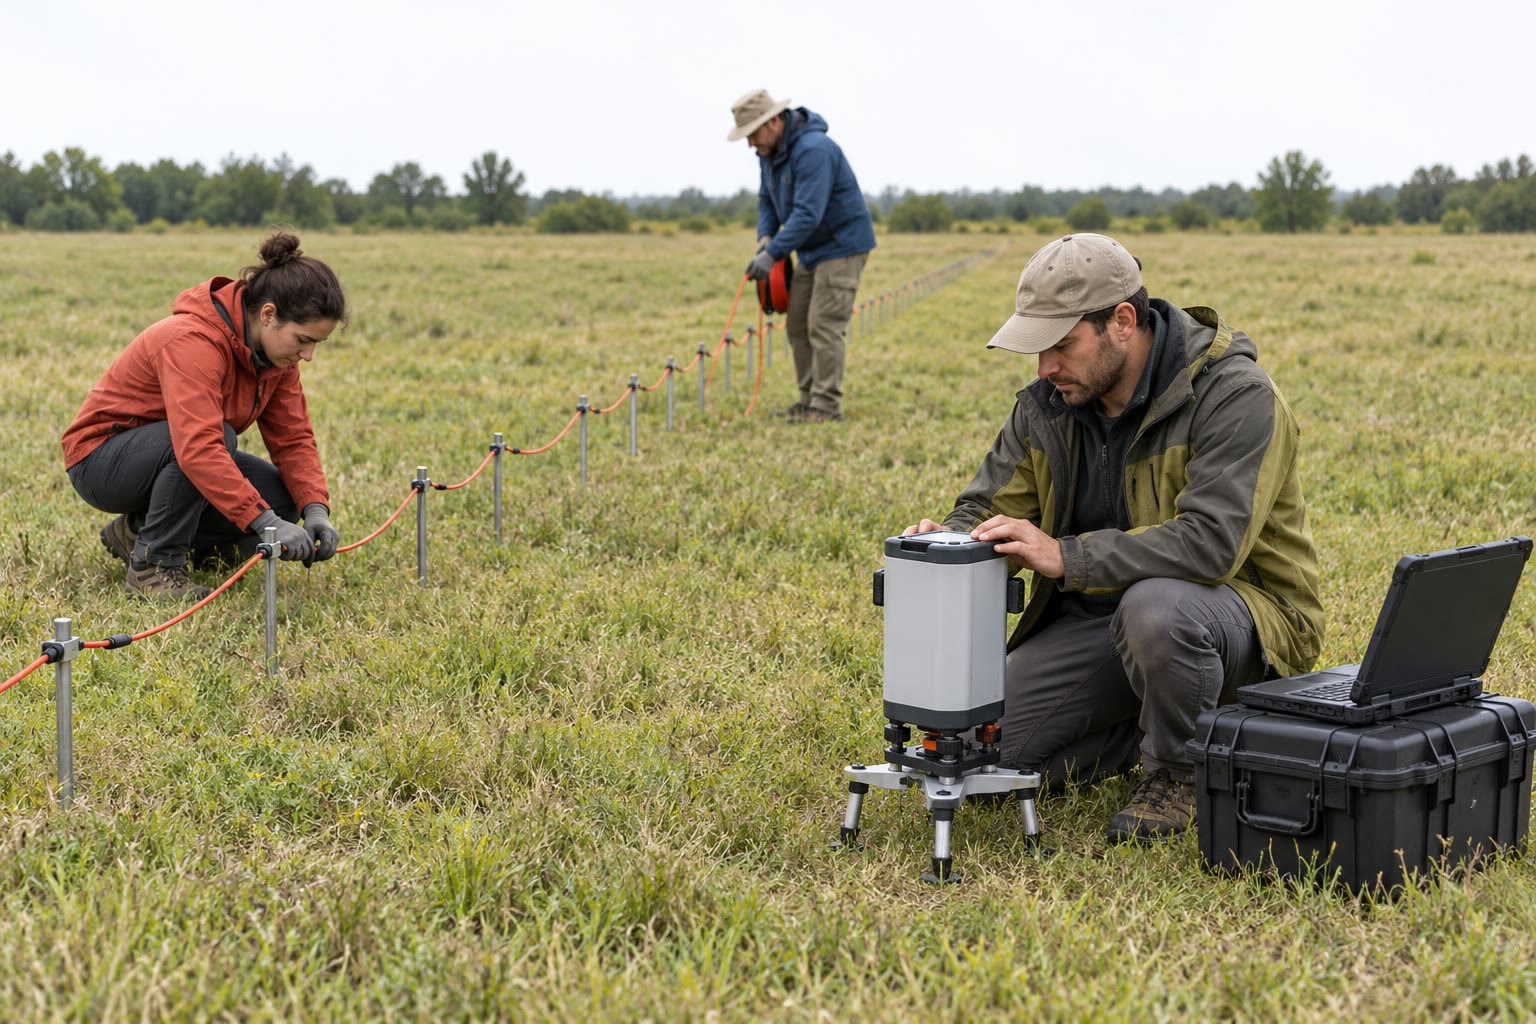
\includegraphics[width=\linewidth]{images/book5/ai/b3-geophysics-crew.jpg}

{\scriptsize Uma equipe de geofísica estende um cabo de resistividade, com um
gravímetro sobre sua base. Ilustração gerada por IA.}
\end{minipage}
\end{inthefield}

\begin{example}[O levantamento Varden]\label{ex:b3:field-lab-methods-3:varden}
O mapa gravimétrico mostra um mínimo fechado de cerca de \qty{-2.3}{\milli\gal}
centrado sobre o granito, alongado norte--sul: o granito menos denso
continua sob a cobertura e é mais longo nessa direção. O mínimo
estende-se até cerca de \qty{1}{km} do afloramento, de modo que o corpo se alarga com
a profundidade. Sua meia-largura fornece uma primeira profundidade para uma esfera equivalente;
modelos com lados verticais e uma base mostram que a base situada entre um
e alguns quilômetros de profundidade explica o pico igualmente bem, dentro de algumas
décimos de miligal, de modo que a base permanece desconhecida---a não unicidade
da seção anterior. No fundo do vale, sobre o granito, a
sondagem começa na resistividade de cascalho seco, cai onde a
corrente entra no aluvião saturado de água e sobe ao longo de uma reta
de inclinação igual a um: uma cobertura condutora sobre uma base altamente resistiva, o
granito, a alguns metros de profundidade. O radar puxado pelo mesmo fundo mostra um
eco plano a cerca de \qty{20}{ns}: o nível freático. E a linha magnética
sobre o flanco oeste da dobra, onde a cobertura é espessa e os
xistos do embasamento jazem a cerca de duzentos metros de profundidade, registra um
máximo simétrico de cerca de \qty{20}{nT} que nenhum mapa explica: um dique máfico,
rico em magnetita, soterrado sob a cobertura; sua direção ao longo do
meridiano magnético é a razão pela qual a anomalia é simétrica. Os geofísicos
o descrevem como um dique de diabásio interrompido na discordância, que a
cobertura do mapa oculta. O problema de fim de semana reduz os dados do
levantamento.
\end{example}
% ledger: gpg:susceptibility, gpg:resistivity, gpg:gpr-table

\section*{Exercícios}

\begin{exercise}[$\star$]\label{exo:b3:field-lab-methods-3:1}
(a)~Que fração de $g = \qty{9.81}{m.s^{-2}}$ equivale a \qty{0.01}{\milli\gal}?
(b)~De quanto deve ser elevado um gravímetro para que sua leitura varie
de \qty{0.01}{\milli\gal} apenas pelo efeito ar livre? (c)~Com os efeitos ar livre e
Bouguer combinados, com a densidade
\qty{2670}{kg.m^{-3}}?
\end{exercise}

\begin{exercise}[$\star$]\label{exo:b3:field-lab-methods-3:2}
Uma esfera de raio \qty{50}{m} e contraste de densidade
\qty{+500}{kg.m^{-3}} tem seu centro a \qty{100}{m} de profundidade. Calcule
a massa excedente, o pico de sua anomalia e a meia-largura $x_{1/2}$.
\end{exercise}

\begin{exercise}[$\star$]\label{exo:b3:field-lab-methods-3:3}
Um arranjo Wenner de espaçamento $a = \qty{10}{m}$ injeta \qty{0.1}{A} e
mede \qty{0.239}{V}. (a)~Calcule o fator geométrico e a
\omterm{def:b3:field-lab-methods-3:resistivity}{resistividade aparente}. (b)~Mostre que um arranjo Schlumberger com $s =
\qty{15}{m}$ e $l = \qty{5}{m}$ tem o mesmo fator geométrico, e
explique por quê.
\end{exercise}

\begin{exercise}[$\star$]\label{exo:b3:field-lab-methods-3:4}
O granito tem $\varepsilon_r = 5$. (a)~Calcule a velocidade do radar. (b)~Uma
fratura está a \qty{10}{m} de profundidade: calcule o tempo de ida e volta de seu eco.
(c)~Com $\sigma = \qty{1}{mS.m^{-1}}$, calcule a profundidade pelicular e a
profundidade útil, de cerca de três profundidades pelicular. (d)~Compare com uma argila úmida de
$\varepsilon_r = 20$ e $\sigma = \qty{10}{mS.m^{-1}}$.
\end{exercise}

\begin{exercise}[$\star\star$]\label{exo:b3:field-lab-methods-3:5}
(a)~Deduza a anomalia de um cilindro horizontal longo de raio $R$ e
contraste de densidade $\Delta\rho$, com eixo na profundidade $z$, a partir da de uma
massa linear, e mostre que $z = x_{1/2}$. (b)~Um cilindro e uma esfera
produzem o mesmo pico e a mesma meia-largura $x_{1/2} = \qty{100}{m}$.
Compare suas profundidades. Qual interpretação fornece o corpo mais profundo?
\end{exercise}

\begin{exercise}[$\star\star$]\label{exo:b3:field-lab-methods-3:6}
A anomalia de Bouguer do modelo do granito de Varden, amostrada a cada
\qty{100}{m} em um mapa de \num{1120} pontos cobrindo $\qty{3.5}{km}
\times \qty{3.2}{km}$, soma \qty{-438}{\milli\gal}. (a)~Aplique
a \cref{prop:b3:field-lab-methods-3:gauss} para estimar o déficit de massa.
(b)~O déficit de massa do modelo é \qty{1.74e11}{kg}. Que fração
o mapa recupera, e onde está o restante?
\end{exercise}

\begin{exercise}[$\star\star$]\label{exo:b3:field-lab-methods-3:7}
(a)~Um dique delgado tem o topo a \qty{30}{m} de profundidade. Usando a regra de três
leituras por meia-largura, em que a meia-largura é a largura total da
anomalia à metade de seu pico, qual espaçamento de estações ela exige? (b)~O
mesmo para um topo a \qty{220}{m} de profundidade. (c)~Por que um único levantamento não
consegue resolver ao mesmo tempo um corpo raso e um profundo, a menos que seja projetado para o
raso?
\end{exercise}

\begin{exercise}[$\star\star$]\label{exo:b3:field-lab-methods-3:8}
Um arenito saturado com água de resistividade \qty{8}{\ohm\metre} tem uma
resistividade de \qty{80}{\ohm\metre}. (a)~Com $a = 1$ e $m = 2$,
calcule sua porosidade. (b)~Repita com $m = 1.8$ e $m = 2.2$. Qual
termo da medição controla a incerteza da porosidade?
\end{exercise}

\begin{exercise}[$\star\star$]\label{exo:b3:field-lab-methods-3:9}
(a)~Calcule os três primeiros termos da série de duas camadas
dada pela \cref{prop:b3:field-lab-methods-3:layers} em $s = 2h_1$ para $k =
\num{0.5}$ e $k = \num{-0.5}$, e as \omterm{def:b3:field-lab-methods-3:resistivity}{resistividades aparentes} que
elas fornecem. (b)~Quais são os limites de $\rho_a/\rho_1$ para $s \ll h_1$ e
$s \gg h_1$? (c)~Quais razões de resistividade $\rho_2/\rho_1$ correspondem a
$k = \pm 0.5$?
\end{exercise}

\begin{exercise}[$\star\star\star$]\label{exo:b3:field-lab-methods-3:10}
(a)~Deduza o fator geométrico do arranjo de Wenner a partir
do \cref{thm:b3:field-lab-methods-3:point-source}. (b)~Deduza o fator geométrico
do arranjo de Schlumberger, e mostre que $\rho_a \to 2\pi s^2(-\mathrm{d}V/
\mathrm{d}r)/I$ quando $l/s \to 0$. (c)~Quanto o fator aproximado
$\pi s^2/(2l)$ superestima o valor exato quando $l = s/10$?
\end{exercise}

\begin{exercise}[$\star\star\star$]\label{exo:b3:field-lab-methods-3:11}
Uma estação está a \qty{50}{m} acima da base. Sua leitura tem precisão de
\qty{0.01}{\milli\gal}, a altura a \qty{5}{cm}; a densidade da
laje é incerta em \qty{100}{kg.m^{-3}}, a \omterm{def:b3:field-lab-methods-3:terrain}{correção de terreno} em
\qty{0.2}{\milli\gal}. (a)~Monte o balanço de erros da anomalia de Bouguer.
anomalia. (b)~Qual termo domina e qual melhoraria para detectar uma
anomalia de \qty{0.1}{\milli\gal}? (c)~Qual é o total sem
o termo de terreno?
\end{exercise}

\begin{exercise}[$\star\star\star$]\label{exo:b3:field-lab-methods-3:12}
Cinco leituras gravimétricas sobre um corpo enterrado, em $x = -600$, $-300$, $0$,
$300$ e \qty{600}{m}, são \num{-0.69}, \num{-2.17}, \num{-4.16},
\num{-2.10} e \qty{-0.73}{\milli\gal}, cada uma com $\sigma =
\qty{0.03}{\milli\gal}$. (a)~Para modelos de esfera centrados sob $x = 0$ nas
profundidades de \num{300}, \num{400} e \qty{500}{m}, escolha a massa que
se ajuste à leitura central e calcule o \omterm{def:b3:field-lab-methods-3:inversion-practice}{desajuste} $\chi^2$ de cada. (b)~Qual
modelo se ajusta aos dados dentro de seus erros? (c)~Um corpo de outra forma poderia
se ajustar igualmente bem? O que decidiria?
\end{exercise}

\section{Problema: Os corpos ocultos das Varden Hills}

\begin{problem}[{Problema de fim de semana --- redução do levantamento Varden}]
\label{pb:b3:field-lab-methods-3:1}
Use $G = \qty{6.674e-11}{m^3.kg^{-1}.s^{-2}}$, o gradiente de ar livre
\qty{0.3086}{\milli\gal.m^{-1}} e o fator de Bouguer
\qty{0.1119}{\milli\gal.m^{-1}} (densidade \qty{2670}{kg.m^{-3}}).

\medskip\noindent\textbf{Parte I --- Um circuito gravimétrico.} Um circuito sobre o
perfil gravimétrico fornece (leituras em miligals após a calibração, alturas
em metros, tempos em horas após 09:00):
\begin{center}
\small
\begin{tabular}{lccccc}
\hline
estação & base & \qty{3.0}{km} & \qty{3.5}{km} & \qty{4.0}{km} & base \\
\hline
tempo & 0 & 0.5 & 0.9 & 1.3 & 2.0 \\
altura & 176.1 & 149.0 & 145.5 & 158.0 & 176.1 \\
leitura & 2846.512 & 2851.075 & 2850.497 & 2849.392 & 2846.708 \\
\hline
\end{tabular}
\end{center}
\begin{enumerate}
\item Calcule a taxa de deriva do circuito.
\item Corrija as três leituras das estações pela deriva e expresse-as
  em relação à base.
\item Aplique as correções de ar livre e de Bouguer para as
  diferenças de altura, e dê a anomalia de Bouguer de cada estação em relação à
  base.
\item A deriva do instrumento sozinho foi \qty{0.040}{\milli\gal.h^{-1}}.
  O que causou o restante da variação na base, e por que ela poderia ser
  removida junto com a deriva?
\item O modelo de onde vêm as leituras fornece as três anomalias
  em relação à base como \num{-0.825}, \num{-2.131} e
  \qty{-0.825}{\milli\gal}. Calcule os erros da redução. As
  alturas da tabela foram arredondadas para \qty{0.1}{m}: que erro esse
  arredondamento pode introduzir, e ele explica os erros?
\item Qual precisão de altura mantém a anomalia reduzida dentro de
  \qty{0.01}{\milli\gal}? Por que os manuais de levantamento pedem
  \qty{3.3}{cm}, um valor mais rigoroso?
\end{enumerate}

\medskip\noindent\textbf{Parte II --- A anomalia do granito.} Ao longo
do perfil a anomalia tem seu mínimo, \qty{-2.293}{\milli\gal}, em
$x = \qty{3.50}{km}$, e cruza metade desse valor em $x = 3.048$ e
\qty{3.952}{km}. O modelo do granito tem um contraste de densidade de
\qty{-130}{kg.m^{-3}}, e o terreno no centro está a \qty{145.5}{m}
acima do nível do mar.
\begin{enumerate}[resume]
\item Calcule a meia-largura $x_{1/2}$ e a profundidade do centro da
  esfera equivalente.
\item Calcule o déficit de massa dessa esfera e seu raio para o
  contraste de densidade do granito. O que há de estranho no resultado?
\item O centro de massa do modelo está a \qty{864}{m} abaixo do terreno e seu
  déficit de massa é \qty{1.74e11}{kg}. Por que a regra da meia-largura fornece um
  corpo mais raso e mais leve?
\item Um cilindro vertical de mesma área que o granito na
  discordância tem raio \qty{461}{m}. Calcule sua anomalia sobre o eixo
  para um topo no terreno e um fundo a \qty{1645}{m} de profundidade, e para uma
  profundidade ilimitada.
\item Encontre, por tentativa ou por resolução, a profundidade do fundo para a qual este
  cilindro fornece a anomalia observada de \qty{-2.29}{\milli\gal}.
\item Calcule a anomalia do cilindro com o topo a \qty{6}{m} de
  profundidade (fundo a \qty{1645}{m}). A gravimetria consegue dizer se o granito chega
  à superfície sob o aluvião?
\end{enumerate}

\medskip\noindent\textbf{Parte III --- O fundo do vale.} A sondagem de Schlumberger
sobre o fundo acima do granito fornece (semiespaçamento $s$ em
metros, $\rho_a$ em \unit{\ohm\metre}):
\begin{center}
\small
\begin{tabular}{lcccccccc}
\hline
$s$ & 1 & 2 & 4 & 6 & 10 & 20 & 30 & 40 \\
$\rho_a$ & 577 & 526 & 387 & 350 & 449 & 821 & 1309 & 1684 \\
\hline
\end{tabular}
\end{center}
Em um perfil de radar ao longo do mesmo fundo, um tubo gera uma hipérbole com
seu vértice em \qty{10.7}{ns} e um tempo de \qty{17.1}{ns} \qty{1}{m}
ao lado; um eco plano chega em \qty{20.0}{ns}.
\begin{enumerate}[resume]
\item Com $s = \qty{20}{m}$, MN tinha \qty{2}{m} de comprimento e a corrente
  \qty{50}{mA}. Calcule o fator geométrico e a tensão medida.
\item Calcule a velocidade do radar, a permissividade relativa do
  aluvião e a profundidade do tubo.
\item O eco plano é o nível freático. Qual é a sua profundidade?
\item Estime a condutância $S$ do aluvião a partir das leituras em
  20, 30 e \qty{40}{m}.
\item O aluvião seco tem \qty{600}{\ohm\metre}, e o aluvião saturado
  \qty{222}{\ohm\metre}. Calcule a espessura do aluvião saturado e a
  profundidade do topo do granito. A estimativa é alta
  ou baixa, e por quê?
\item A água subterrânea tem \qty{20}{\ohm\metre}. Calcule a porosidade do
  aluvião pela \omterm{prop:b3:field-lab-methods-3:archie}{lei de Archie} com $m = 2$, e o intervalo de $m$
  entre \num{1.3} e \num{2.8}.
\end{enumerate}

\medskip\noindent\textbf{Parte IV --- A linha magnética.} A linha segue
para leste a partir de $x = \qty{1.70}{km}$, uma estação a cada \qty{50}{m} e a cada
dois minutos; a estação-base registrou nos mesmos minutos. As leituras,
menos \qty{48000}{nT}, são:
\begin{center}
\small
\setlength{\tabcolsep}{3.5pt}
\begin{tabular}{lccccccccccc}
\hline
$x$ (km) & 1.70 & 1.75 & 1.80 & 1.85 & 1.90 & 1.95 & 2.00 & 2.05 & 2.10 & 2.15 & 2.20 \\
linha & 3.4 & 4.8 & 6.3 & 8.1 & 10.3 & 12.8 & 15.8 & 19.2 & 22.9 & 26.2 & 28.0 \\
base & 0.0 & 0.7 & 1.5 & 2.2 & 2.9 & 3.6 & 4.3 & 5.0 & 5.7 & 6.4 & 7.0 \\
\hline
$x$ (km) & 2.25 & 2.30 & 2.35 & 2.40 & 2.45 & 2.50 & 2.55 & 2.60 & 2.65 & 2.70 & \\
linha & 27.7 & 25.8 & 23.3 & 20.9 & 19.0 & 17.6 & 16.6 & 15.9 & 15.5 & 15.2 & \\
base & 7.6 & 8.2 & 8.8 & 9.4 & 9.9 & 10.4 & 10.9 & 11.3 & 11.7 & 12.1 & \\
\hline
\end{tabular}
\end{center}
O campo principal é \qty{48000}{nT}, com inclinação de \ang{65}.
\begin{enumerate}[resume]
\item Aplique a \omterm{def:b3:field-lab-methods-3:magnetic}{correção diurna} e forneça a anomalia corrigida em
  cada estação.
\item Mostre que, sem a correção, a anomalia nunca cai até a metade
  de seu pico no lado leste.
\item Localize o pico e os dois pontos em que a anomalia corrigida vale
  a metade do pico, por interpolação linear, e calcule a meia-largura.
\item A anomalia é simétrica. O que isso diz sobre a direção do
  corpo, e que tipo de corpo a regra da meia-largura supõe?
\item Calcule o produto $\kappa t$ da suscetibilidade pela espessura.
  Se o dique é um diabásio de suscetibilidade \num{0.03}, qual é a sua
  espessura?
\item As estações estavam suficientemente próximas?
\item Forneça a profundidade do topo do dique oculto abaixo do solo, até
  a dezena de metros mais próxima, e compare-a com a profundidade da
  discordância no modelo geológico da região, \qty{222}{m} neste
  ponto.
\end{enumerate}
\end{problem}
% ledger: gpg:grav-survey, gpg:mag-field, keys:archie
